%%%%%%%%%%%%%%%%%%%%%%%%%%%%%%%%%%%%%%%%%%%%%%
%                                            %
%   W Z O R Z E C   S P R A W O Z D A N I A  %
%                                            %
%%%%%%%%%%%%%%%%%%%%%%%%%%%%%%%%%%%%%%%%%%%%%%


\documentclass[12pt,a4paper]{article}
%\documentclass[12pt,a4paper,twoside]{article}

\usepackage{amsmath,amssymb}
\usepackage[utf8]{inputenc}                                      
\usepackage[OT4]{fontenc}      
%\usepackage[T1]{fontenc}                            
\usepackage[polish]{babel}                           
\selectlanguage{polish}
\usepackage{indentfirst} 
\usepackage[dvips]{graphicx}
\usepackage{tabularx}
\usepackage{color}
\usepackage{hyperref} 
\usepackage{fancyhdr}
\usepackage{listings}
\usepackage{booktabs}
\usepackage{ifpdf}
\usepackage{mathtext} % polskie znaki w trybie matematycznym
%\makeindex  % utworzenie skorowidza (w dokumencie pdf)
\usepackage{lmodern}
%\usepackage[osf]{libertine}
\usepackage{filecontents}
\usepackage{ifthen}

%\usepackage[cp1250]{inputenc}
\usepackage{graphicx} 

\usepackage{tikz}
\usetikzlibrary{arrows}


\newcounter{nextYear}
\setcounter{nextYear}{\the\year}
\stepcounter{nextYear}

% rozszerzenie nieco strony
%\setlength{\topmargin}{-1cm} \setlength{\textheight}{24.5cm}
%\setlength{\textwidth}{17cm} \addtolength{\hoffset}{-1.5cm}
%\setlength{\parindent}{0.5cm} \setlength{\footskip}{2cm}
%\linespread{1.2} % odstep pomiedzy wierszami


%%%% ZYWA PAGINA %%%%%%%%%%%
\newcommand{\tl}[1]{\textbf{#1}} 
\pagestyle{fancy}
\renewcommand{\sectionmark}[1]{\markright{\thesection\ #1}}
\fancyhf{} % usuwanie bieżących ustawień
\fancyhead[LE,RO]{\small\bfseries\thepage}
\fancyhead[LO]{\small\bfseries\rightmark}
\fancyhead[RE]{\small\bfseries\leftmark}
\renewcommand{\headrulewidth}{0.5pt}
\renewcommand{\footrulewidth}{0pt}
\addtolength{\headheight}{0.5pt} % pionowy odstęp na kreskę
\fancypagestyle{plain}{%
\fancyhead{} % usuń p. górne na stronach pozbawionych numeracji
\renewcommand{\headrulewidth}{0pt} % pozioma kreska
}

%%%%%   LISTINGI %%%%%%%%
% ustawienia listingu programow

\lstset{%
language=C++,%
commentstyle=\textit,%
identifierstyle=\textsf,%
keywordstyle=\sffamily\bfseries, %
%captionpos=b,%
tabsize=3,%
frame=lines,%
numbers=left,%
numberstyle=\tiny,%
numbersep=5pt,%
breaklines=true,%
morekeywords={pWezel,Wezel,string,ref,params_result},%
escapeinside={(*@}{@*)},%
%basicstyle=\footnotesize,%
%keywords={double,int,for,if,return,vector,matrix,void,public,class,string,%
%float,sizeof,char,FILE,while,do,const}
}
%%%%%%%%%%%%%%%%%%%%%%%%%%%%%%%%%%%%%%%%%%%%%%%%%%%%%%%%%%%%%%%%%%%%%%%

%%%%%%%%%  NOTKI NA MARGINESIE %%%%%%%%%%%%%
% mala zmiana sposobu wyswietlania notek bocznych
\let\oldmarginpar\marginpar
\renewcommand\marginpar[1]{%
  {\linespread{0.85}\normalfont\scriptsize%
\oldmarginpar[\hspace{1cm}\begin{minipage}{3cm}\raggedleft\scriptsize\color{black}\textsf{#1}\end{minipage}]%    left pages
{\hspace{0cm}\begin{minipage}{3cm}\raggedright\scriptsize\color{black}\textsf{#1}\end{minipage}}% right pages
}%
}
% % % % % % % % % % % % % % % % % % % % % % % % % % % % % % % %

%%%% WYSWIETLANIE AKTUALNEGO ROKU AKADEMICKIEGO %%%%%%%%%%%
\newcounter{rok}
\newcommand{\rokakademicki}{%
   \setcounter{rok}{\number\year}%
   \ifthenelse{\number\month<10}%
   {\addtocounter{rok}{-1}}% rok akademicki zaczal sie w pazdzierniku poprzedniego roku
   {}%                       rok akademicki zaczyna sie w pazdzierniku tego roku
   \arabic{rok}/\addtocounter{rok}{1}\arabic{rok}
}
%%%%%%%%%%%%%%%%%%%%%%%%%%%%%%%%%%%%%%%


%%%% LISTA UWAG %%%%%%%%%
\usepackage{color}
\definecolor{brickred}      {cmyk}{0   , 0.89, 0.94, 0.28}

\makeatletter \newcommand \kslistofremarks{\section*{Uwagi} \@starttoc{rks}}
\newcommand\l@uwagas[2]
{\par\noindent \textbf{#2:} %\parbox{10cm}
   {#1}\par} \makeatother


\newcommand{\ksremark}[1]{%
   {{\color{brickred}{[#1]}}}%
   \addcontentsline{rks}{uwagas}{\protect{#1}}%
}

\newcommand{\comma}{\ksremark{przecinek}}
\newcommand{\nocomma}{\ksremark{bez przecinka}}
\newcommand{\styl}{\ksremark{styl}}
\newcommand{\ortografia}{\ksremark{ortografia}}
\newcommand{\fleksja}{\ksremark{fleksja}}
\newcommand{\pauza}{\ksremark{pauza `--', nie dywiz `-'}}
\newcommand{\kolokwializm}{\ksremark{kolokwializm}}
\newcommand{\cytowanie}{\ksremark{cytowanie}}

%%%%%%%%%%%%%%%%%%%%%%%%%
%%%%%%%%%%%%%%%%%%%%%%%%%
%%%%%%%%%%%%%%%%%%%%%%%%%
%%%%%%%%%%%%%%%%%%%%%%%%%
%%%%%%%%%%%%%%%%%%%%%%%%%
%%%%%%%%%%%%%%%%%%%%%%%%%
%%%%%%%%%%%%%%%%%%%%%%%%%
%%%%%%%%%%%%%%%%%%%%%%%%%
%%%%%%%%%%%%%%%%%%%%%%%%%
%%%%%%%%%%%%%%%%%%%%%%%%%
%%%%%%%%%%%%%%%%%%%%%%%%%
%%%%%%%%%%%%%%%%%%%%%%%%%



% autor:
\fancyhead[RE]{\small\bfseries Michał Pawłowski} % autor sprawozdania



%%%%%%%%%%% NO I ZACZYNA SIE SPRAWOZDANIE %%%%%%%%%%%

\begin{document}
\frenchspacing
\thispagestyle{empty}
\begin{center}
{\Large\sf Politechnika Śląska   % Alma Mater

Wydział Informatyki, Elektroniki i Informatyki

}

\vfill

 

\vfill\vfill

{\Huge\sffamily\bfseries Programowanie Komputerów\par}  

\vfill\vfill

{\LARGE\sf Space Invaders}   


\vfill \vfill\vfill\vfill

%%%%%%%%%%%%%%%%%%%%%%%%%%%%





\begin{tabular}{ll}
	\toprule
	autor                       & Michał Pawłowski    \\
	prowadzący                  &  dr hab. inż., prof. Roman Starosolski   \\
	rok akademicki              & \rokakademicki         \\
	kierunek                    & informatyka            \\
	rodzaj studiów              & SSI                    \\
	semestr                     & 4                      \\
	termin laboratorium         & wtorek 13:30\\
	sekcja                      & 1                    \\
	termin oddania sprawozdania & 2021-05-13            \\
	\bottomrule
	                            &
\end{tabular}

\end{center}
%%% koniec strony  tytulowej

%%%%%%%%%%%%%%%%%%%%%%%%%%%%%%%%%%%%%%%%%%%%%%%%%%%%%%%%%%%%%%%%%%%%%%%%%
\cleardoublepage
%%%%%%%%%%%%%%%%%%%%%%%%%%%%%%%%%%%%%%%%%%%%%%%%%%%%%%%%%%%%%%%%%%%%%%%%%

%%%%%%%%%%%%%%%%%%%%%%%%%%%%%%%%%%%%%%%%%%%%%%%%%%%%%%%%%%%%%%%%%%%%%%%%%
\section{Temat}
Gra Space Invaders wydana w 1978 to jedna z pierwszych gier komputerowych. Pierwotnie stworzona na dedykowane automaty do gry a następnie przeniesiona na urządzenia Atari 2600. Realizowany projekt polega na implementacji tej klasycznej gry 2D w języku C++.

%%%%%%%%%%%%%%%%%%%%%%%%%%%%%%%%%%%%%%%%%%%%%%%%%%%%%%%%%%%%%%%%%%%%%%%%%
\section{Analiza tematu}
Założenia gry są następujące. Kosmici poruszają się poziomo z jednakową prędkością, gdy znajdą się przy krawędzi planszy przenoszą się poziom niżej. Istnieje jednak pewna szansa, iż pojedynczy kosmita odłączy się od grupy i zaatakuje sam. Dodatkowo kosmici w sposób losowy oddają strzały w kierunku gracza. Nad grupą atakujących kosmitów od czasu do czasu przelatuje UFO, którego zestrzelenie gwarantuje dodatkowe punkty. Gracz przesuwa poziomo działo, którym stara się zestrzelić wszystkich kosmitów. Może się on schronić się za osłony, te jednak niszczą się wraz z zablokowanymi strzałami. Trafienie kosmity oznacza jego eliminację (usunięcie z planszy). Gracz otrzymuje 10, 20 lub 30 punktów za eliminację kosmity w zależności od jego rodzaju oraz 150 punktów i dodatkowe życie za eliminację UFO. Każdy poziom oznacza nową falę przeciwników, która różni się liczbą kosmitów. Gra kończy się gdy poziom życia gracza spadnie do 0 lub gdy kosmici dotrą na wysokość gracza, czyli do dołu planszy.

Program ma być uruchamiany w trybie okienkowym oraz wykorzystywać klawiaturę jako urządzenie wejścia. Dlatego wykorzystana została biblioteka SFML, która pozwala w prosty sposób zarządzać urządzeniami I/O oraz renderowaniem obrazu.

%%%%%%%%%%%%%%%%%%%%%%%%%%%%%%%%%%%%%%%%%%%%%%%%%%%%%%%%%%%%%%%%%%%%%%%%%
\section{Specyfikacja zewnętrzna}
\label{sec:sp:zewnetrzna}
\subsection{Instrukcja dla użytkownika}
Skompilowany program został umieszczony w folderze razem z plikami niezbędnymi do poprawnego działania. Aby uruchomić program należy wykonać plik \lstinline|spaceinvaders.exe|

Po uruchomieniu programu pojawia się plansza startowa. Gra rozpoczyna się po naciśnięciu przycisku \texttt{enter}. Podczas gry użytkownik przesuwa działo w poziomie za pomocą klawiszy \texttt{left} i \texttt{right} oraz oddaje strzały za pomocą klawisza \texttt{spacja}. Informacje o bieżącym wyniku, poziomie oraz zdrowiu gracza wyświetlane są w górze ekranu. Po zakończeniu gry na ekranie pojawia się informacyjna plansza z wynikiem uzyskanym oraz najlepszym w historii. Użytkownik może rozpocząć nową grę klawiszem \texttt{enter} lub wyjść z programu za pomocą \texttt{esc}.

Jeżeli podczas otwierania programu lub w czasie jego działania wykryty zostanie błąd, program automatycznie zakończy swoje działanie a informacja o nim zostanie wypisana na strumień błędów np.

\begin{verbatim}
ERROR[2]: Unable to open texture.
\end{verbatim}


Uwaga! Do poprawnego działania programu niezbędny jest pakiet Microsoft Visual C++ 2015-2019 Redistributable (x64) w wersji 14.23.27820
\subsection{Zrzuty ekranu}
\begin{figure}[h]
\centering
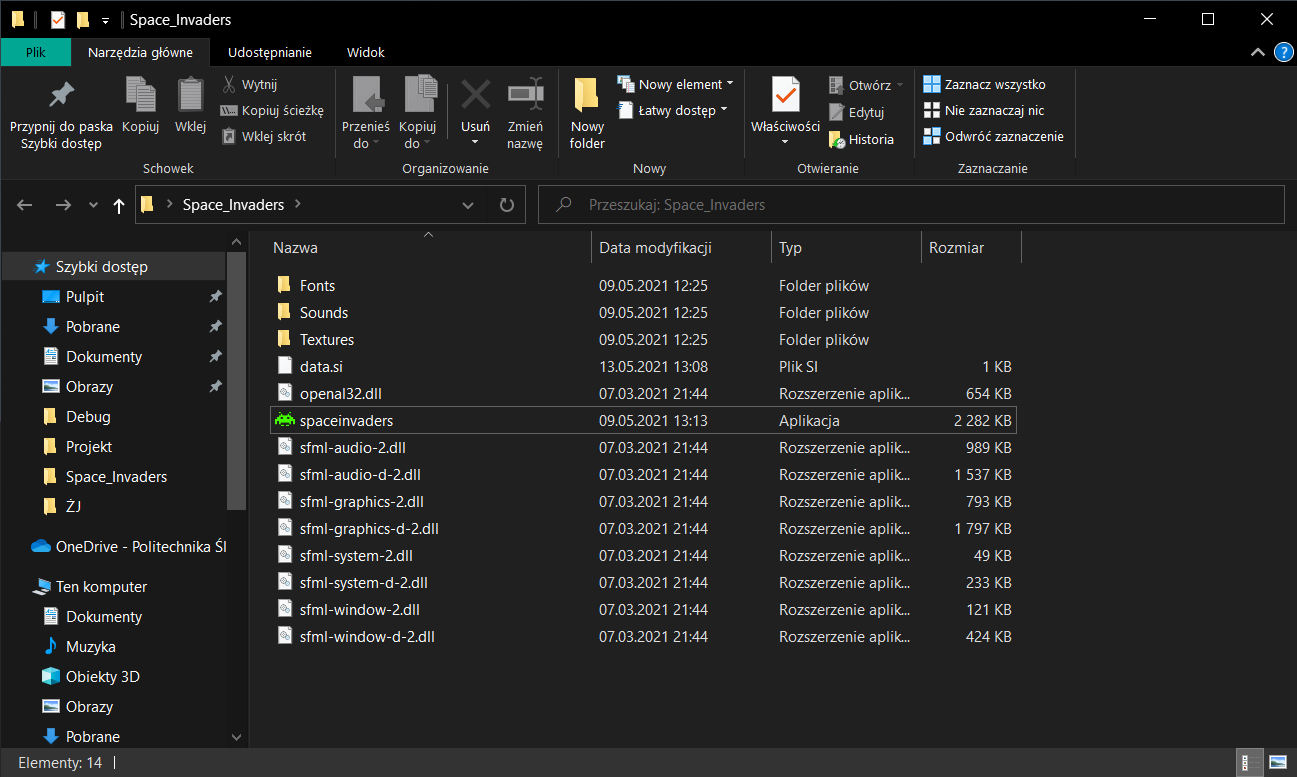
\includegraphics[width=14cm]{katalog}
\caption{ \centering Katalog zawierający pliki gry.}
\label{fig:katalog}
\end{figure}

\clearpage

\begin{figure}[h]
\centering
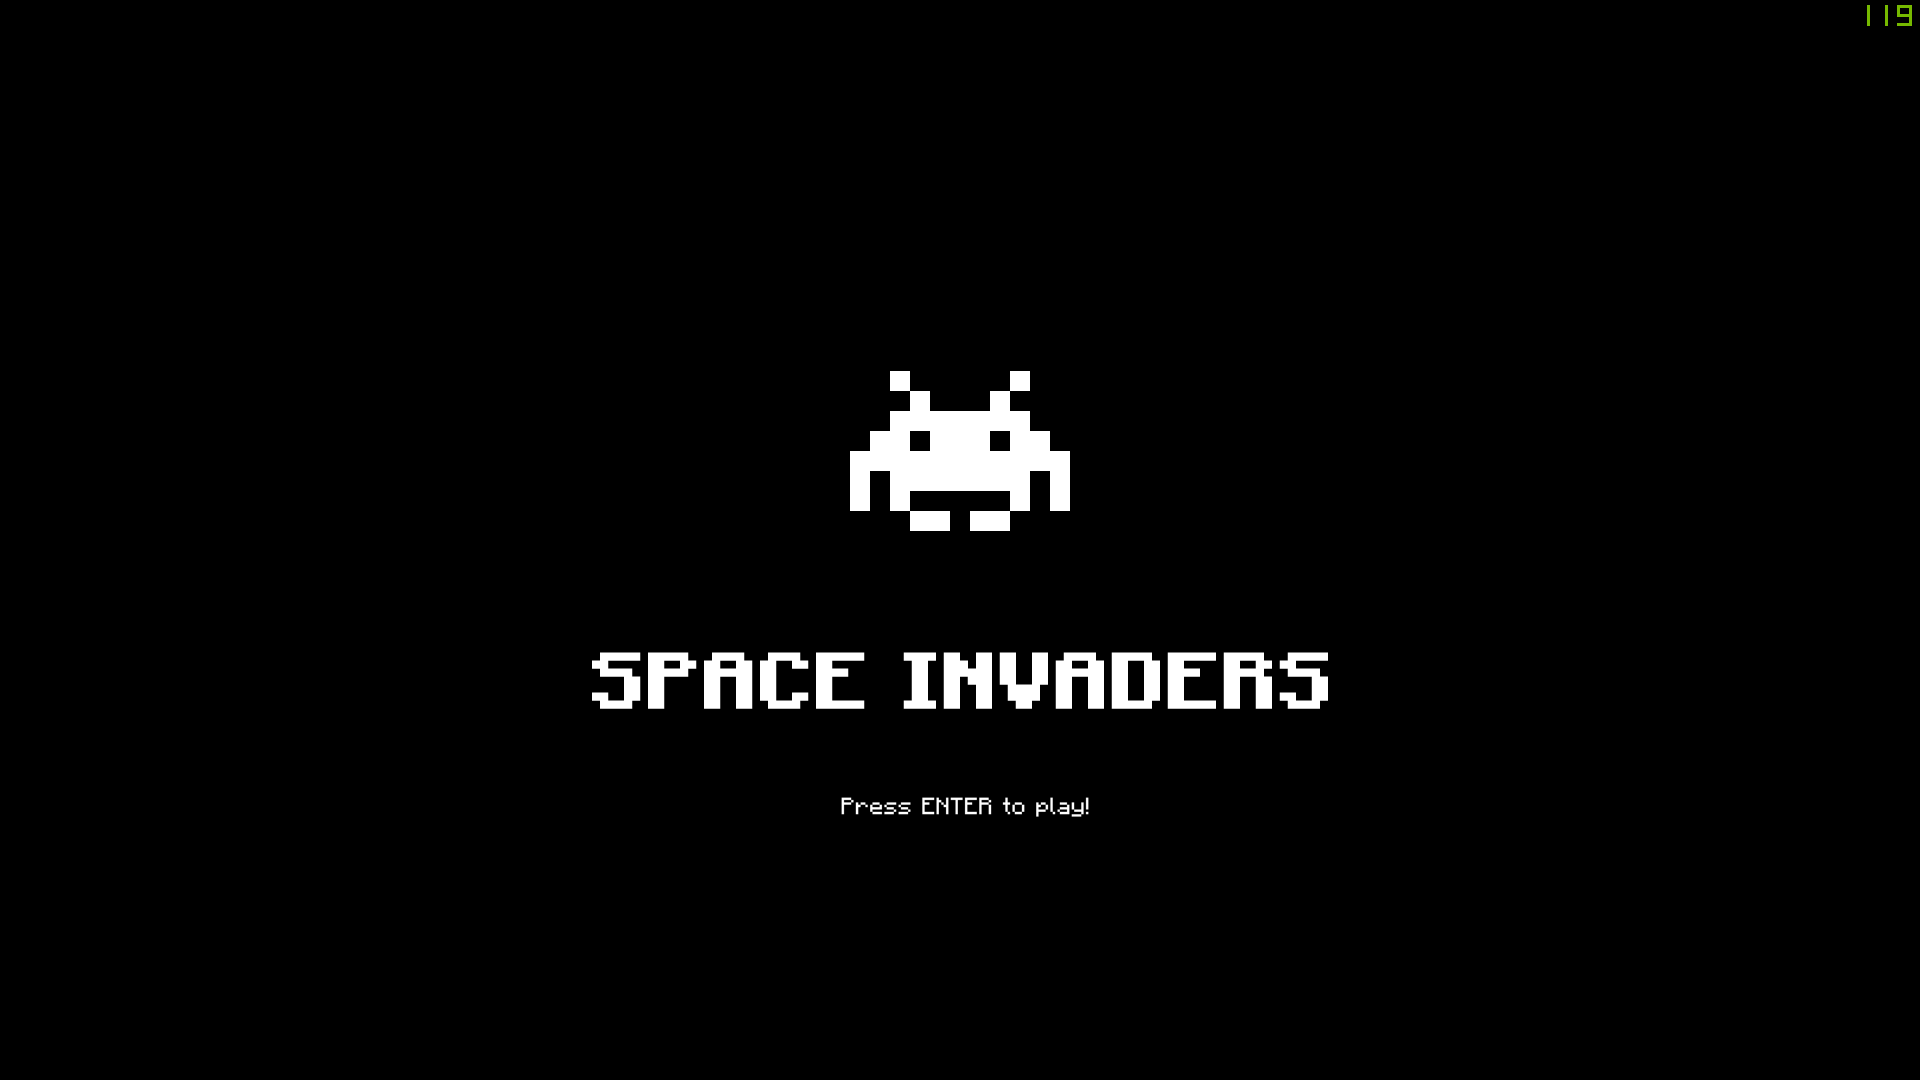
\includegraphics[width=11.8cm]{start}
\caption{ \centering Plansza startowa wyświetlana po uruchomieniu programu.}
\label{fig:start}
\end{figure}

\begin{figure}[h]
\centering
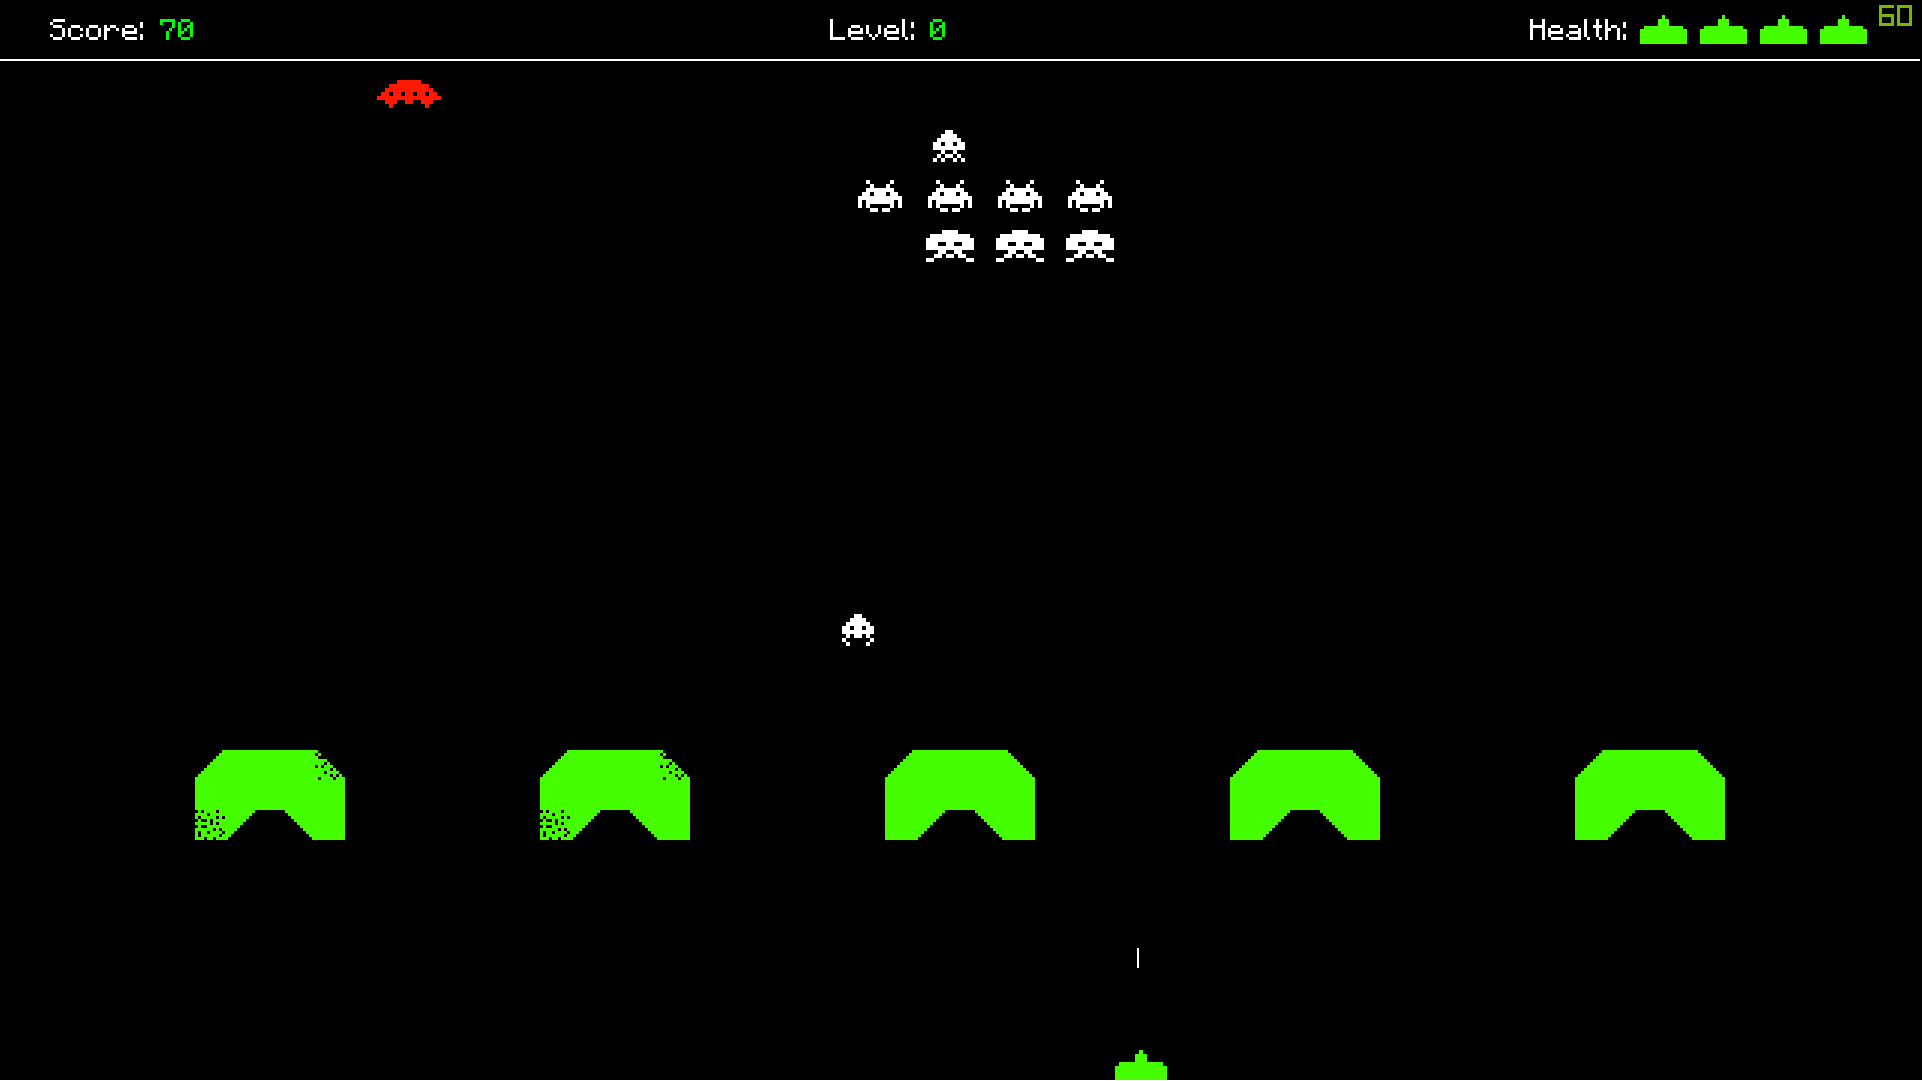
\includegraphics[width=11.8cm]{interface}
\caption{ \centering Interfejs gry.}
\label{fig:interface}
\end{figure}

\clearpage

\begin{figure}[h]
\centering
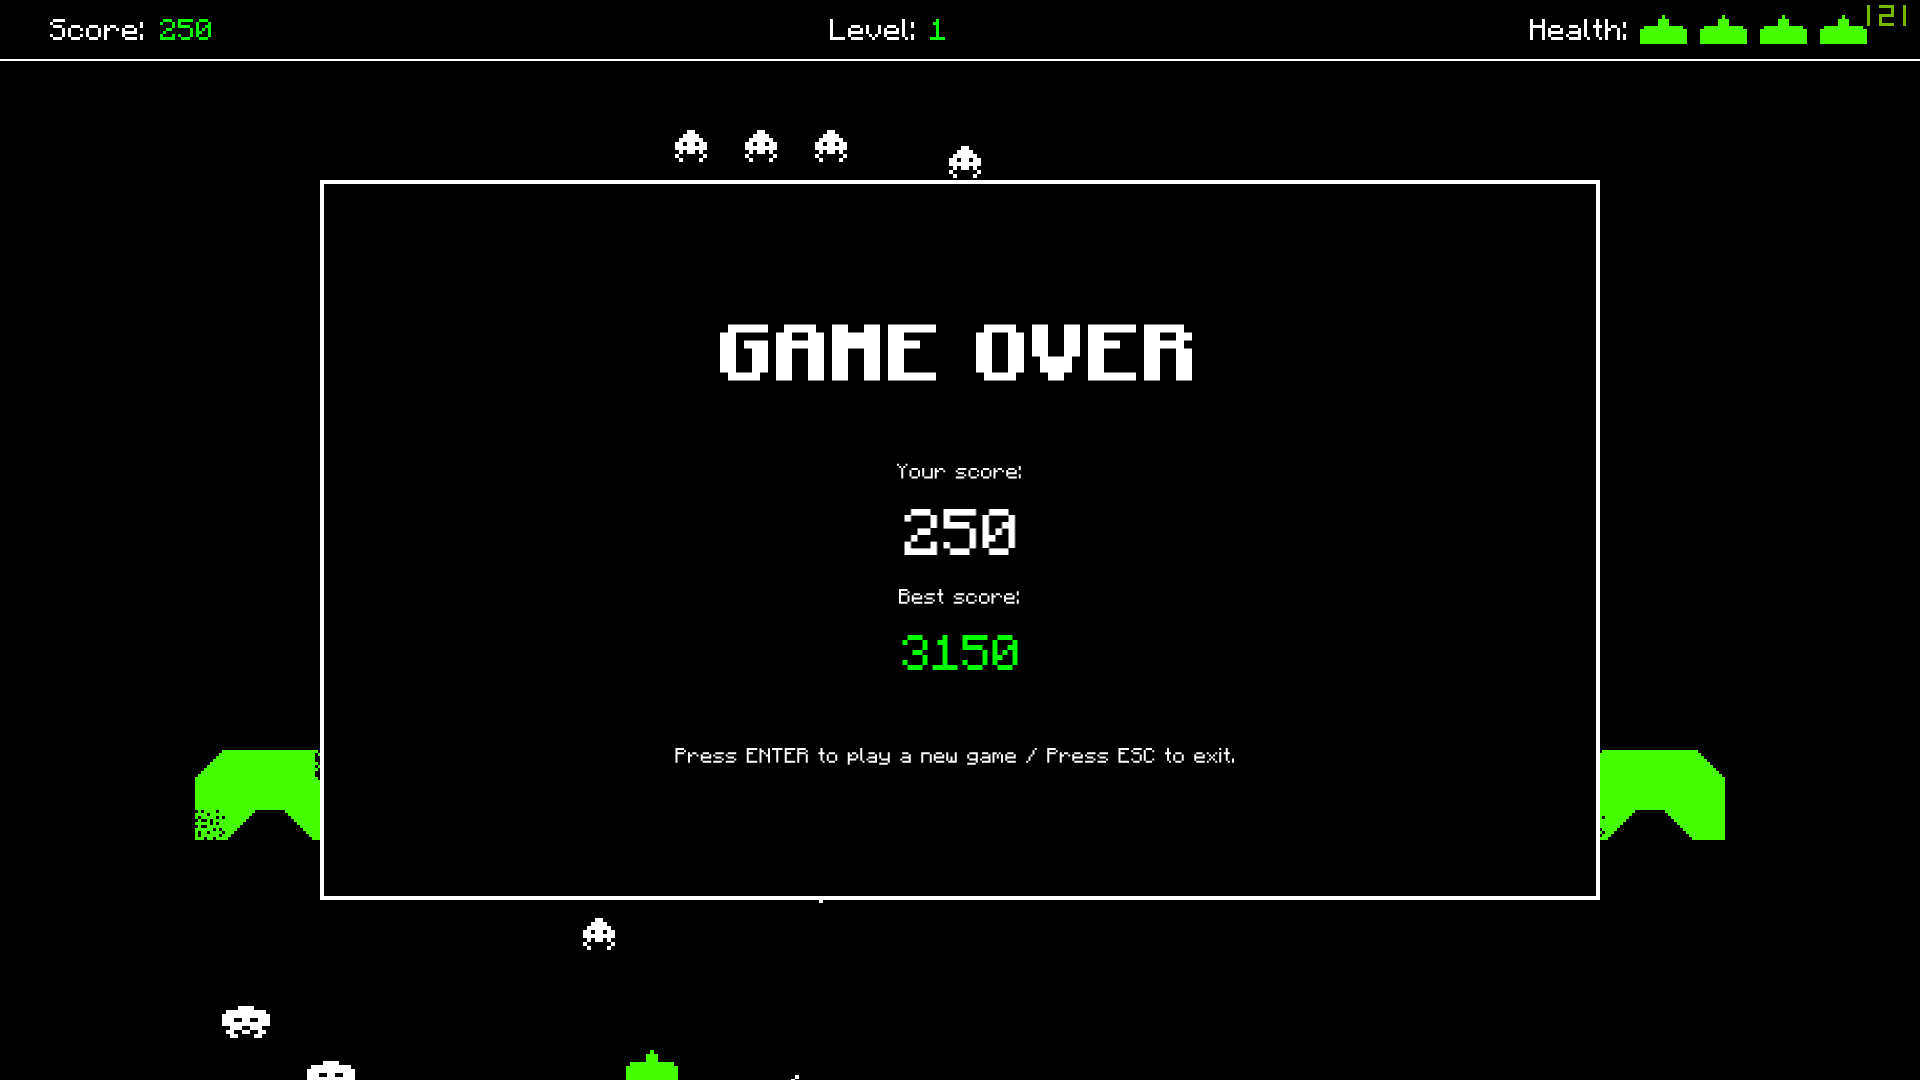
\includegraphics[width=11.8cm]{end}
\caption{ \centering Plansza końcowa wyświetlana po zakończeniu gry.}
\label{fig:end}
\end{figure}


%%%%%%%%%%%%%%%%%%%%%%%%%%%%%%%%%%%%%%%%%%%%%%%%%%%%%%%%%%%%%%%%%%%%%%%%%
\section{Specyfikacja wewnętrzna}\label{sec:sp-wew}

\subsection{Omówienie najważniejszych klas}
W programie możemy wyróżnić co najmniej kilka najważniejszych klas. Silnik gry został zadeklarowany w klasie \lstinline|Game|. Zawiera ona w sobie wszystkie obiekty, tworzone na potrzeby działania programu. Znajdziemy w niej zatem zarówno obiekty definiujące konkretne elementy gry jak i obiekty klas pochodzących z biblioteki SFML, odpowiedzialnych za otwieranie programu w oknie, renderowania itp. Metody zadeklarowane w tej klasie to zbiór metod stanowiących główną mechanikę gry. 

Zadaniem klasy \lstinline|Wall| jest poprawne skonstruowanie i przechowywanie tablicy obiektów klasy \lstinline|Block|, która definiuje pojedynczy blok osłony za którą może się chować gracz. Klasa \lstinline|Walls| przechowuje w wektorze obiekty \lstinline|Wall| oraz zarządza nimi.

\lstinline|Unit| to abstrakcyjna klasa bazowa po której dziedziczą wszystkie klasy definiujące jednostki (postacie) z gry. Zawiera ona głównie pola i metody wywodzące się z biblioteki SFML. Bezpośrednio po tej klasie dziedziczy \lstinline|Player| oraz \lstinline|Ufo|. W pierwszej klasie zaimplementowane są metody umożliwiające interakcję z użytkownikiem, czyli sterowanie i strzelanie. Druga klasa definiuje obiekt UFO, który od czasu do czasu pojawia się na ekranie. Trzecią klasą dziedziczącą po \lstinline|Unit| jest klasa abstrakcyjna \lstinline|Enemy|. Stanowi ona klasę bazową dla klas \lstinline|Squid|, \lstinline|Crab|  i \lstinline|Octopus|.  Klasy pochodne w różny sposób deklarują metody wirtualne klasy bazowej, tak by zachowanie na planszy przeciwników innych klasy było zróżnicowane. Obiekty tych klas znajdują się w strukturze danych zawartej w klasie \lstinline|Enemies|. 

Klasa \lstinline|Collisions| implementuje metody niezbędne do wykrywania kolizji pomiędzy wszelkimi obiektami.
\subsection{Hierarchia klas}

\begin{figure}[h]
\centering
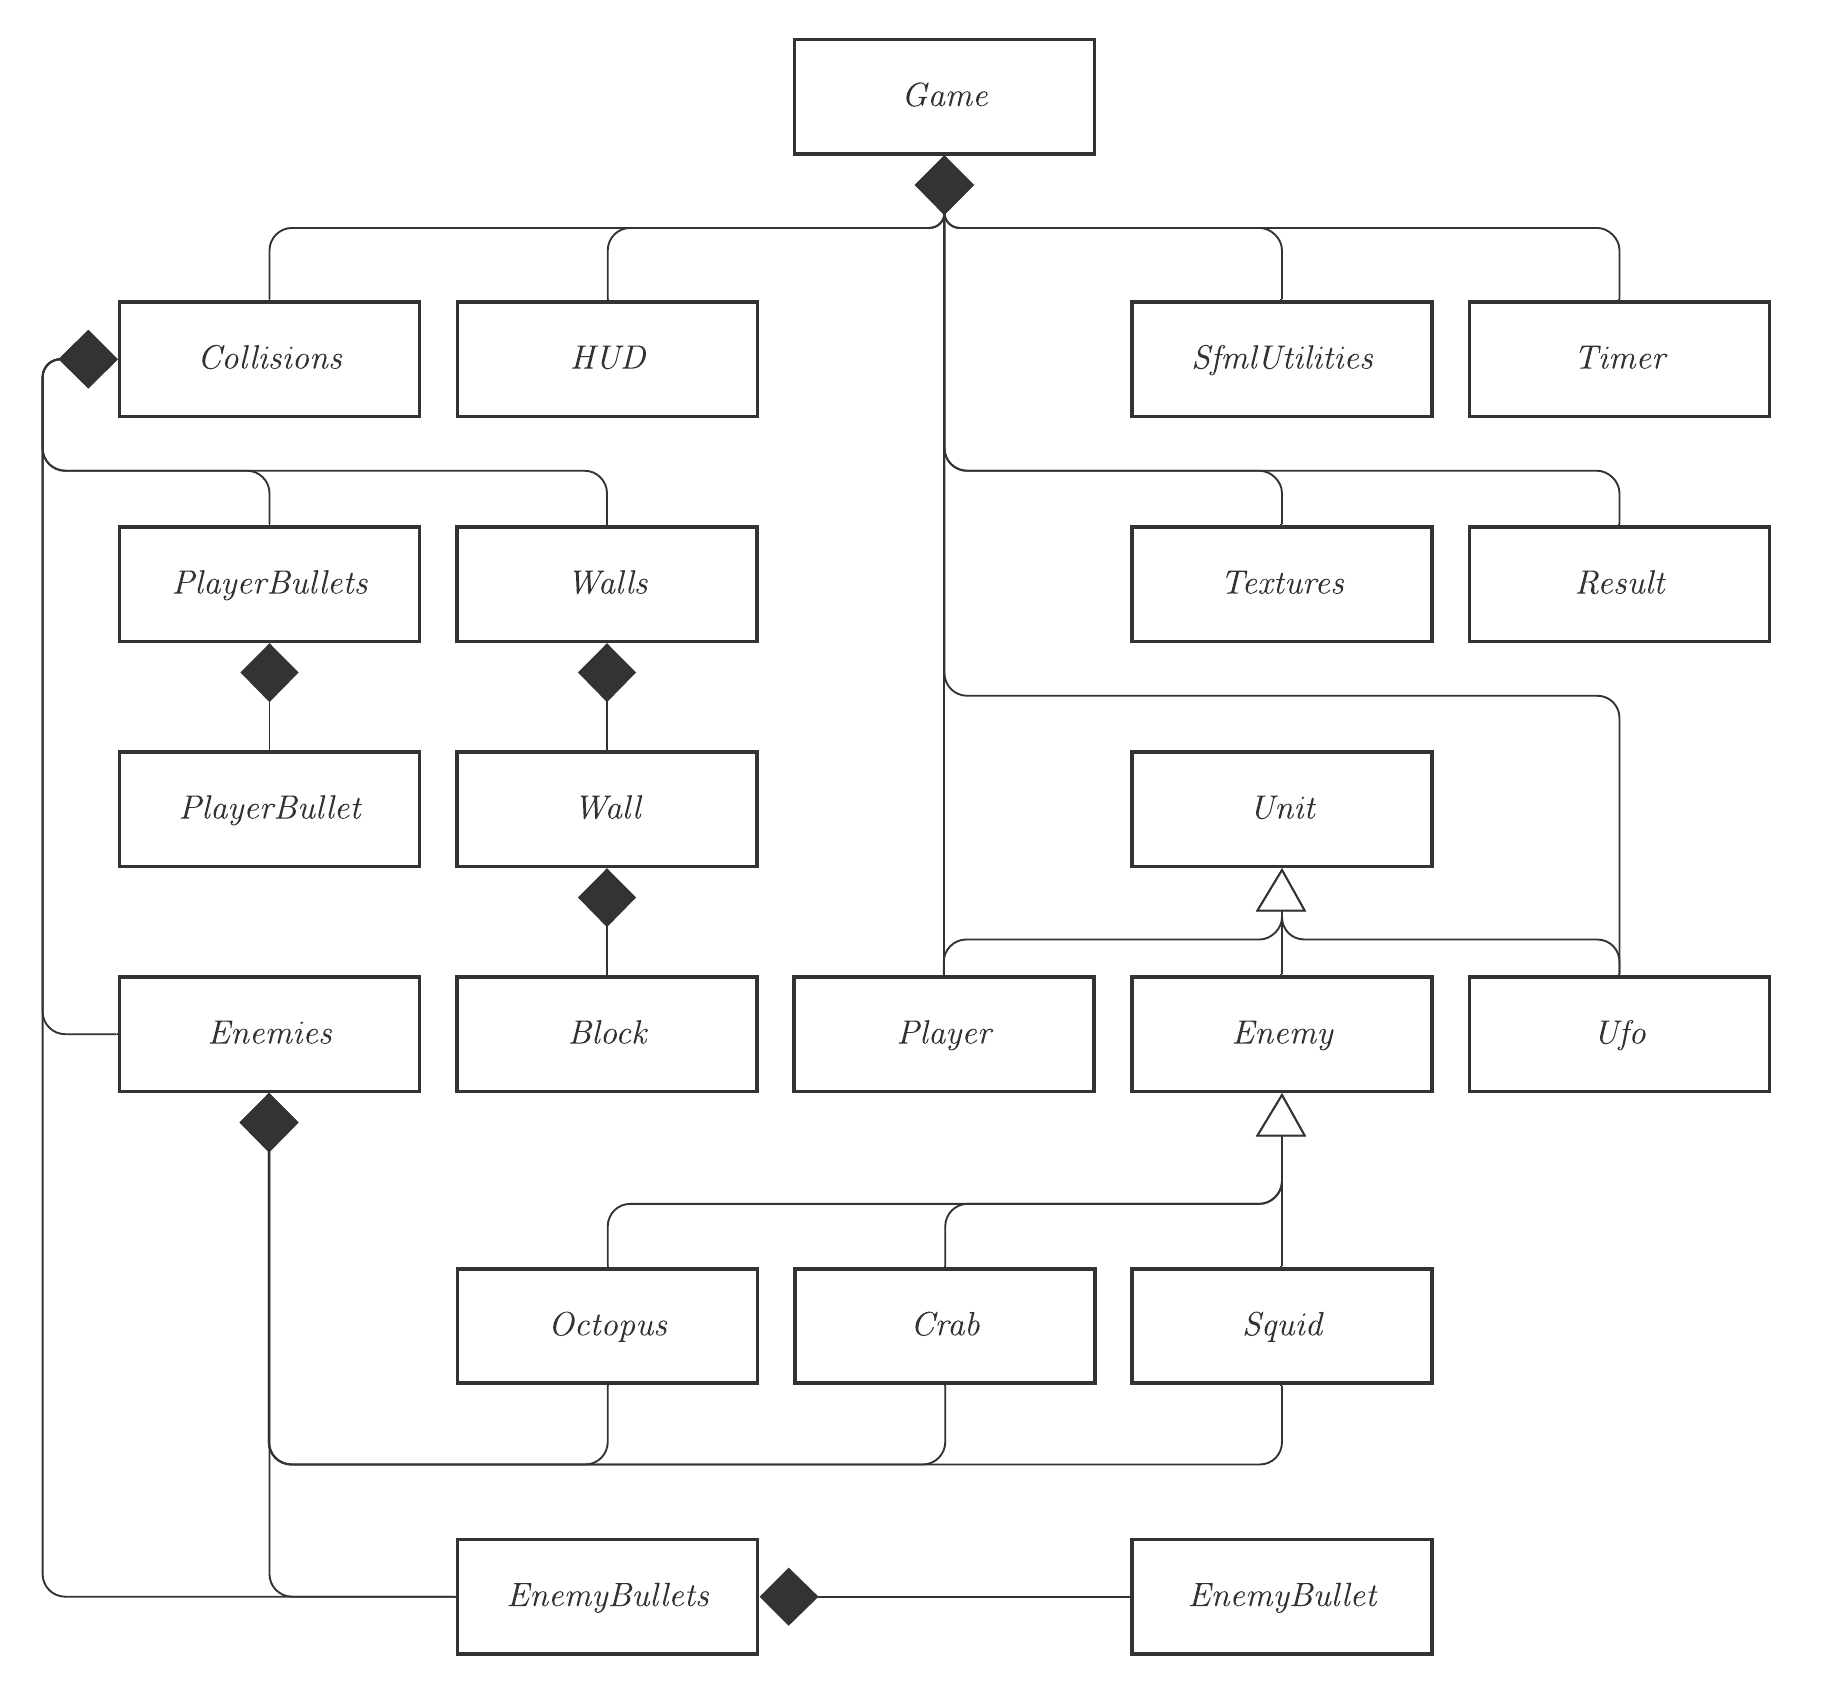
\includegraphics[width=14cm]{ULM}
\caption{ \centering Diagram klas ULM.}
\label{fig:interface}
\end{figure} 

\subsection{Szczegółowy opis klas i metod}

Szczegółowy opis klas i metod zostanie wygenerowany przy pomocy Doxygen'a i załączony do finalnego sprawozdania.
 
\subsection{Struktury danych}
Ilość przeciwników jest zmienna w zależności od danego poziomu. Dlatego też obiekty klas pochodnych wirtualnej klasy \lstinline|Enemy| są przechowywane w liście list znajdującej się w obiekcie klasy \lstinline|Enemies|. Jest to największa struktura danych w programie. Oprócz niej wykorzystywane są pomniejsze struktury danych takie jak: mapy (do przechowywania wskaźników na tekstury) oraz wektory (do przechowywania obiektów klas \lstinline|Wall|, \lstinline|Block|, \lstinline|PlayerBullet|, \lstinline|EnemyBullet|.

Wszystkie struktury danych zostały stworzone w oparciu o kontenery STL typu \lstinline|list|, \lstinline|vector| czy \lstinline|map|.

\begin{figure}[h]
\centering
\begin{tikzpicture}

\node[rectangle, draw, minimum width=3cm, minimum height = 1cm] (L1) at (-5,0) {$List$};
	\node[rectangle, draw, minimum size=1cm] (M1) at (-1,0) {$E$};
	\node[rectangle, draw, minimum size=1cm] (M2) at (2,0) {$E$};
	\node[rectangle, draw, minimum size=1cm] (M3) at (5,0) {$E$};
\node[rectangle, draw, minimum width=3cm, minimum height = 1cm] (L2) at (-5,-1.5) {$List$};
	\node[rectangle, draw, minimum size=1cm] (M4) at (-1,-1.5) {$E$};
	\node[rectangle, draw, minimum size=1cm] (M5) at (2,-1.5) {$E$};
	\node[rectangle, draw, minimum size=1cm] (M6) at (5,-1.5) {$E$};
\node[rectangle, draw, minimum width=3cm, minimum height = 1cm] (L3) at (-5,-3) {$List$};
	\node[rectangle, draw, minimum size=1cm] (M7) at (-1,-3) {$E$};
	\node[rectangle, draw, minimum size=1cm] (M8) at (2,-3) {$E$};
	\node[rectangle, draw, minimum size=1cm] (M9) at (5,-3) {$E$};


\draw[>=latex,->] (L1) -- (L2);
\draw[>=latex,->] (L2) -- (L3);
\draw[>=latex,->] (L1) -- (M1);
\draw[>=latex,->] (M1) -- (M2);
\draw[>=latex,->] (M2) -- (M3);
\draw[>=latex,->] (L2) -- (M4);
\draw[>=latex,->] (M4) -- (M5);
\draw[>=latex,->] (M5) -- (M6);
\draw[>=latex,->] (L3) -- (M7);
\draw[>=latex,->] (M7) -- (M8);
\draw[>=latex,->] (M8) -- (M9);


\end{tikzpicture}
\caption{ \centering Przykładowy schemat listy list.}

\label{fig:graf}
\end{figure} 



\subsection{Ogólny schemat działania programu}
Program rozpoczyna się od utworzenia obiektu klasy \lstinline|Game|. W trakcie konstrukcji tworzone są również wszystkie zadeklarowane w niej obiekty. W obiekcie klasy \lstinline|Enemies| zainicjowana zostaje struktura danych zawierająca obiekty klasy \lstinline|Enemy|. Jej elementy stopniowo są usuwane wraz z eliminacjami dokonanymi przez gracza. Po przejściu do kolejnego poziomu struktura zostaje zainicjowana na nowo, tym razem z inną liczbą elementów. Program działa w nieskończonej pętli, dopóki okno aplikacji pozostaje otwarte, wywołując metody \lstinline|update()| oraz \lstinline|render()|. Pierwsza z nich odpowiedzialna jest za sczytanie sygnałów urządzeń wejściowych oraz wprowadzanie zmian w obiektach, tak by symulować postęp gry. Druga natomiast odpowiada za wyświetlanie zmian w oknie aplikacji. Przed zakończeniem działania programu zwolniona zostaje zaalokowana pamięć.

\subsection{Biblioteki zewnętrzne i techniki obiektowe}
Program opiera się o technikę programowania obiektowego. Wykorzystane zostały m.in.: klasy, klasy abstrakcyjne z metodami wirtualnymi, dziedziczenie, hermetyzacja, polimorfizm. W programie zawarte zostały również elementy języka C++ przedstawione na laboratoriach: mechanizm wyjątków, kontenery STL, algorytmy i iteratory STL oraz szablony funkcji. Program wykorzystuje bibliotekę Simple and Fast Multimedia Library (SFML).


\section{Testowanie}
Program był testowany zarówno na bieżąco podczas programowania jak i w finalnej wersji przez niezależne osoby. Podczas programowania wykryto typowe błędy programistyczne  takie jak m.in.: wyjście po za zakres, odwołanie do usuniętego obiektu. Wykryte błędy skorygowano. Przetestowano wszystkie możliwe kolizje. Wynikające z nich usuwanie obiektów ze struktur danych, nie generuje problemów ani wycieków pamięci. Finalny program został przetestowany przez 3 niezależne osoby. Podczas testów nie wykryły one żadnych błędów. 

\section{Wnioski}
Stworzenie prostej gry 2D daje możliwość przećwiczenia oraz wykazania się umiejętnościami programowania obiektowego. W porównaniu do projektów z poprzednich semestrów, wykorzystanie kontenerów STL zamiast struktur samodzielnie zaimplementowanych znacznie upraszcza i przyspiesza proces pisania programu. Wykorzystanie zewnętrznej biblioteki SFML pozwoliło na stworzenie programu w trybie okienkowym skupiając się na paradygmatach programowania obiektowego bez zagłębiania się w dokumentację OpenGL.

\section{Link do repozytorium}
https://github.com/polsl-aei-pk4/0fa12ac6-gr21-repo/tree/main/Projekt
 
\cleardoublepage

\rule{0cm}{0cm}

\vfill

\begin{center}
\Huge\bfseries Dodatek\\Szczegółowy opis typów i~funkcji\par
\end{center}

\vfill 

\rule{0cm}{0cm}

\end{document}
